\documentclass[11pt,spanish]{article} % Tipo y tamaño de letra del documento.

\input{preamble.tex}
\usepackage{booktabs} % Para tablas profesionales

\input{author.tex}

\headheight=14pt
\linespread{1.3}
\author{\namestudent}
\pagestyle{fancy}
\fancyhf{}%
\fancyfoot[R]{ \namestudent \\ \rolusm}
\fancyfoot[L]{Campus \campus}
\fancyfoot[C]{\thepage}
\rhead{\sem}
\lhead{INF-221}
\renewcommand{\headrulewidth}{0.4pt}
\renewcommand{\footrulewidth}{0.4pt}
\newbool{programs}
\boolfalse{programs}
\chead{REPORTE TAREA \tnum~}

\title{
  \huge
  \textbf{REPORTE TAREA \tnum~ \\ ALGORITMOS Y COMPLEJIDAD} \\[1ex]
  \emph{\textquote{¿Quién ganará? Greedys vs Dinámico vs Bruto.}}
  }

\date{
  \small
  \today\\
  \currenttime
}

\begin{document}
\maketitle
\thispagestyle{fancy}
\vspace{-1.0\baselineskip}

\section{Descripción de los Algoritmos}

En esta sección se detallan los cuatro enfoques algorítmicos implementados para resolver el problema \textbf{AniMarathon}, enfocado en la selección óptima de capítulos de anime bajo restricciones de tiempo ($M$) y energía ($E$).

\subsection{Algoritmo de Fuerza Bruta}
El algoritmo de Fuerza Bruta resuelve el problema mediante una exploración exhaustiva de todas las combinaciones factibles de prefijos para los $n$ animes. Dado que para cada anime $i$ solo se puede ver un prefijo consecutivo de capítulos $k_i \in [0, q_i]$, el espacio de búsqueda total consiste en elegir un vector de prefijos $(k_1, k_2, \dots, k_n)$. El algoritmo utiliza una función recursiva de backtracking con poda de factibilidad: en el paso $i$, se evalúa cada posible longitud de prefijo $k_i$ para el anime $i$. Si en algún punto el tiempo acumulado supera $M$ o la energía acumulada supera $E$, esa rama del espacio de búsqueda es podada inmediatamente, ya que los costos son monótonamente crecientes. Al alcanzar una hoja factible (decisión para los $n$ animes), se actualiza la máxima satisfacción obtenida, sumando el bono $b_i$ únicamente si el anime correspondiente fue completado en su totalidad ($k_i = q_i$).

\subsection{Heurísticas Greedy}
Se implementaron dos estrategias heurísticas greedy que difieren sustancialmente en su criterio de decisión local y granularidad.

\subsubsection{Greedy 1: Densidad de Satisfacción Global por Anime}
El criterio local de esta heurística evalúa la eficiencia global de cada anime de manera independiente. Para cada anime $i$, se determina qué longitud de prefijo $k \in [1, q_i]$ maximiza el ratio de satisfacción total (incluyendo el bono $b_i$ si $k = q_i$) respecto al costo total de recursos (tiempo más energía). Es decir, para cada anime $i$ se encuentra el candidato óptimo según la densidad local:
\[
\text{densidad}(i) = \max_{1 \le k \le q_i} \left\{ \frac{\sum_{j=1}^k v_{i,j} + \mathbb{I}(k = q_i) \cdot b_i}{\sum_{j=1}^k t_{i,j} + \sum_{j=1}^k c_{i,j}} \right\}
\]
donde $\mathbb{I}$ es la función indicadora de completación. Los animes candidatos con sus respectivos prefijos óptimos se ordenan de forma descendente por su densidad. Luego, el algoritmo realiza una selección greedy recorriendo la lista ordenada e incorporando el bloque completo del prefijo elegido para cada anime, siempre y cuando no se superen las restricciones globales $M$ y $E$.

\subsubsection{Greedy 2: Selección Marginal por Capítulo}
A diferencia de Greedy 1, esta heurística toma decisiones a nivel de capítulo individual y de forma incremental. Se mantiene un puntero $k_i$ para cada anime $i$, indicando cuántos capítulos se han seleccionado actualmente. En cada iteración, el algoritmo evalúa cuál de los siguientes capítulos factibles (es decir, el capítulo $k_i$ de cada anime $i$ que cumpla con los límites restantes de tiempo y energía) aporta la mayor satisfacción marginal por unidad de costo de recursos (duración + energía). El ratio marginal para el anime $i$ se calcula como:
\[
\text{ratio\_marginal}(i) = \frac{v_{i, k_i} + \mathbb{I}(k_i = q_i - 1) \cdot b_i}{t_{i, k_i} + c_{i, k_i}}
\]
Se selecciona el capítulo con el mayor ratio, se actualizan los recursos acumulados, se incrementa $k_i$ y se repite el proceso hasta que ningún capítulo adicional sea factible dentro de los límites de tiempo y energía. Esta heurística es más flexible, ya que permite intercalar capítulos de diferentes animes y puede detenerse en fracciones de anime si se agotan los recursos.

\subsection{Programación Dinámica}
Para resolver el problema de manera óptima, se modela el problema como una variante del problema de la mochila bidimensional con grupos disjuntos (Grouped 2D Knapsack).

Definimos formalmente el estado de la programación dinámica como:
\begin{center}
$DP[i][m][e]$: La máxima satisfacción que se puede obtener considerando los primeros $i$ animes ($0 \le i \le n$), utilizando exactamente $m$ minutos de tiempo ($0 \le m \le M$) y $e$ unidades de energía ($0 \le e \le E$).
\end{center}

Sean $prefT[i][k]$, $prefC[i][k]$ y $prefV[i][k]$ el tiempo, energía y satisfacción acumulados para el prefijo de tamaño $k$ del anime $i$ ($0 \le k \le q_i$). La ecuación de recurrencia que gobierna los estados de transición está dada por:
\[
DP[i][m][e] = \max_{0 \le k \le q_i} \left\{ DP[i-1][m - prefT[i][k]][e - prefC[i][k]] + prefV[i][k] + \mathbb{I}(k = q_i) \cdot b_i \right\}
\]
sujeto a que $m - prefT[i][k] \ge 0$ y $e - prefC[i][k] \ge 0$.

Los casos base se definen como:
\[
DP[0][m][e] = \begin{cases} 
0 & \text{si } m = 0 \text{ y } e = 0 \\
-\infty & \text{en otro caso}
\end{cases}
\]

Para optimizar el uso de memoria de $O(n \cdot M \cdot E)$ a $O(M \cdot E)$, dado que el estado $i$ solo depende del estado anterior $i-1$, implementamos la DP utilizando una tabla auxiliar temporal para almacenar los nuevos estados durante la transición de cada grupo, evitando así la reincorporación de capítulos del mismo anime en el mismo paso.

\section{Análisis de Complejidad}

A continuación se presenta y justifica el análisis de la complejidad temporal y espacial para los cuatro algoritmos implementados, expresado en la notación asintótica Big-O. Definimos $n$ como la cantidad de animes, $Q$ como el número promedio de capítulos por anime ($Q = \frac{1}{n}\sum_{i=1}^n q_i$), $M$ como el límite de tiempo y $E$ como el límite de energía.

\subsection{Fuerza Bruta}
\begin{itemize}
    \item \textbf{Complejidad Temporal:} $O(Q^n)$. Para cada uno de los $n$ animes se tienen $q_i + 1 \approx Q$ decisiones posibles de prefijo. Dado que la búsqueda explora todas las combinaciones en forma de árbol de decisión, el número total de estados hoja factibles es el producto de las decisiones: $\prod_{i=1}^n (q_i + 1) \approx O(Q^n)$, lo cual representa una complejidad exponencial que se vuelve intratable para $n > 10$.
    \item \textbf{Complejidad Espacial:} $O(n \cdot Q)$. El espacio está dominado por la representación en memoria de las series y capítulos de entrada, más el costo del stack de recursión que tiene una profundidad máxima de $O(n)$ correspondiente al número de animes.
\end{itemize}

\subsection{Greedy 1: Densidad Global}
\begin{itemize}
    \item \textbf{Complejidad Temporal:} $O(n \cdot Q + n \log n)$. Para cada anime $i$, se evalúan sus $q_i$ prefijos en tiempo lineal para hallar el candidato de mayor densidad, costando $O(\sum q_i) = O(n \cdot Q)$ en total. Posteriormente, ordenar los $n$ candidatos por su densidad toma $O(n \log n)$ mediante algoritmos como Quicksort. Finalmente, la iteración greedy toma $O(n)$.
    \item \textbf{Complejidad Espacial:} $O(n \cdot Q)$. Requiere almacenar los datos de los capítulos de entrada y una estructura lineal de tamaño $n$ para los candidatos greedy.
\end{itemize}

\subsection{Greedy 2: Selección Marginal}
\begin{itemize}
    \item \textbf{Complejidad Temporal:} $O(n^2 \cdot Q)$. En el peor de los casos, la heurística selecciona todos los capítulos disponibles en la entrada, resultando en un máximo de $\sum q_i = n \cdot Q$ iteraciones del ciclo principal. En cada paso de decisión, se busca el elemento máximo comparando el ratio marginal de los $n$ animes en $O(n)$ pasos.
    \item \textbf{Complejidad Espacial:} $O(n \cdot Q)$. No almacena estructuras dinámicas complejas adicionales a los datos de entrada y a un vector contador de tamaño $n$ para rastrear el progreso de los prefijos.
\end{itemize}

\subsection{Programación Dinámica}
\begin{itemize}
    \item \textbf{Complejidad Temporal:} $O(n \cdot Q \cdot M \cdot E)$. La DP procesa de forma secuencial los $n$ animes. Para cada uno, recorre el espacio completo de estados bidimensionales $(M+1) \times (E+1)$. En cada estado, se evalúan las transiciones asociadas a las $q_i + 1$ longitudes de prefijo factibles del anime actual. Así, el número total de operaciones es proporcional a $\sum_{i=1}^n (q_i + 1) \cdot M \cdot E \approx O(n \cdot Q \cdot M \cdot E)$.
    \item \textbf{Complejidad Espacial:} $O(n \cdot Q + M \cdot E)$. Gracias al uso de una estructura de almacenamiento optimizada con una matriz auxiliar temporal para las transiciones del grupo $i$, el espacio ocupado por la tabla DP se reduce a una matriz de dimensiones $(M+1) \times (E+1)$, lo que equivale a un costo espacial de $O(M \cdot E)$ además del espacio de entrada $O(n \cdot Q)$.
\end{itemize}

\section{Entorno Experimental}

\subsection{Hardware y Software}
Las simulaciones y experimentos de medición se ejecutaron en una máquina bajo el sistema operativo Linux con un procesador Intel(R) Core(TM) i7-10750H CPU @ 2.60GHz y 16 GB de memoria RAM. Los ejecutables se compilaron bajo el compilador \texttt{g++} versión 11.4.0, habilitando optimizaciones agresivas mediante la bandera \texttt{-O3} y utilizando el estándar de C++ \texttt{-std=c++17}.

\subsection{Casos de Prueba (Datasets)}
Se generó una suite experimental de 27 casos de prueba estructurados en tres categorías:
\begin{itemize}
    \item \textbf{Casos Pequeños ($n \in \{3, 5, 8\}$):} Diseñados para verificar la corrección del algoritmo de Fuerza Bruta en comparación con la Programación Dinámica.
    \item \textbf{Casos Medianos ($n \in \{20, 40, 80\}$):} Orientados a medir la brecha de optimización (calidad de solución) de los Greedy en relación al óptimo teórico.
    \item \textbf{Casos Grandes ($n \in \{100, 150, 200\}$):} Destinados a evaluar el comportamiento límite en tiempo y memoria de los algoritmos de Programación Dinámica y Greedy.
\end{itemize}
Para cada tamaño $n$, se crearon 3 réplicas aleatorias con un promedio de $Q \in [2, 10]$ episodios por anime. Las restricciones de recursos se ajustaron de manera competitiva en el rango de $M \in [0.35 \times T_{total}, 0.65 \times T_{total}]$ y $E \in [0.35 \times C_{total}, 0.65 \times C_{total}]$, asegurando escenarios altamente restringidos y no triviales.

\section{Resultados y Análisis}

A continuación se presentan los resultados experimentales agregados a través de las réplicas y tamaños evaluados.

\subsection{Resultados Cuantitativos Obtenidos}
La Tabla~\ref{tab:resultados_muestra} resume el rendimiento de los cuatro algoritmos sobre instancias representativas del experimento.

\begin{table}[H]
\centering
\caption{Comparativa de Rendimiento y Satisfacción sobre casos muestra ($i=1$)}
\label{tab:resultados_muestra}
\resizebox{\textwidth}{!}{%
\begin{tabular}{@{}lcrrrrrr@{}}
\toprule
\textbf{Instancia} & \textbf{Algoritmo} & \textbf{Satisfacción} & \textbf{Calidad (\%)} & \textbf{Tiempo (ms)} & \textbf{Memoria (MB)} \\ \midrule
\textbf{testcases\_3\_1}  
 & Fuerza Bruta       & 528      & 100.00\% & 5.91      & 3.50 \\
 & Greedy 1           & 243      & 46.02\%  & 2.89      & 3.50 \\
 & Greedy 2           & 526      & 99.62\%  & 2.96      & 3.50 \\
 & Prog. Dinámica     & 528      & 100.00\% & 4.03      & 3.75 \\ \midrule
\textbf{testcases\_20\_1} 
 & Fuerza Bruta       & N/A      & N/A      & N/A       & N/A  \\
 & Greedy 1           & 3\,717   & 92.81\%  & 2.98      & 3.50 \\
 & Greedy 2           & 3\,625   & 90.51\%  & 2.09      & 3.50 \\
 & Prog. Dinámica     & 4\,005   & 100.00\% & 212.35    & 30.42 \\ \midrule
\textbf{testcases\_100\_1}
 & Fuerza Bruta       & N/A      & N/A      & N/A       & N/A  \\
 & Greedy 1           & 22\,458  & 77.77\%  & 2.01      & 3.63 \\
 & Greedy 2           & 27\,157  & 94.04\%  & 2.22      & 3.63 \\
 & Prog. Dinámica     & 28\,878  & 100.00\% & 32\,348.90 & 1\,173.38 \\ \midrule
\textbf{testcases\_200\_1}
 & Fuerza Bruta       & N/A      & N/A      & N/A       & N/A  \\
 & Greedy 1           & 42\,910  & 83.92\%  & 4.17      & 3.63 \\
 & Greedy 2           & 47\,556  & 93.01\%  & 10.23     & 3.63 \\
 & Prog. Dinámica     & 51\,132  & 100.00\% & 256\,579.55& 3\,942.13 \\ \bottomrule
\end{tabular}%
}
\end{table}

\subsection{Análisis de Tiempo de Ejecución}
La Figura~\ref{fig:performance} muestra las curvas de tiempo de ejecución promedio de los algoritmos en función de la cantidad de animes.

\begin{figure}[H]
    \centering
    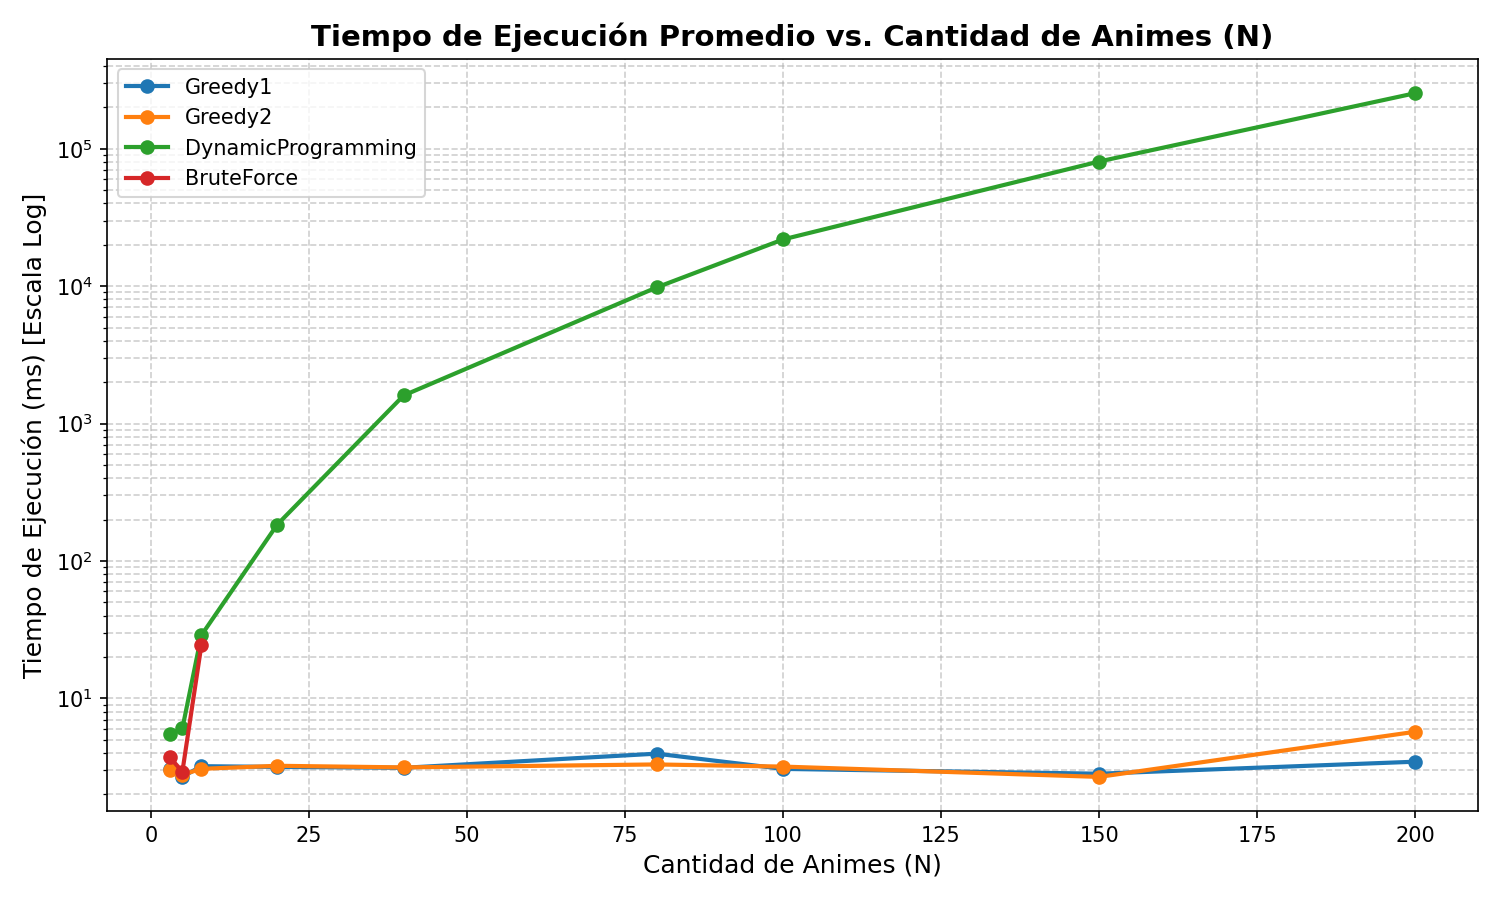
\includegraphics[width=0.70\textwidth]{../code/implementation/data/plots/performance_vs_n.png}
    \caption{Tiempo de ejecución promedio (ms) vs. Cantidad de animes ($N$) en escala logarítmica.}
    \label{fig:performance}
\end{figure}

Como se observa en el gráfico y la tabla, la Fuerza Bruta escala de manera exponencial e interrumpe su ejecución para $n > 10$. El tiempo de ejecución de la Programación Dinámica crece de manera polinomial conforme $N, M, E$ aumentan, alcanzando un promedio de 256.58 segundos para $N=200$. Este comportamiento experimental coincide con la complejidad teórica $O(n \cdot Q \cdot M \cdot E)$, donde los límites de recursos $M$ y $E$ crecen proporcionalmente con $n$ en la generación de pruebas. En contraparte, ambos algoritmos Greedy mantienen tiempos insignificantes e inferiores a los 11 ms, comportándose de manera extremadamente ágil incluso sobre las instancias más grandes.

\subsection{Análisis de Uso de Memoria}
La Figura~\ref{fig:memory} expone el consumo de memoria física (RSS) medido para cada uno de los métodos.

\begin{figure}[H]
    \centering
    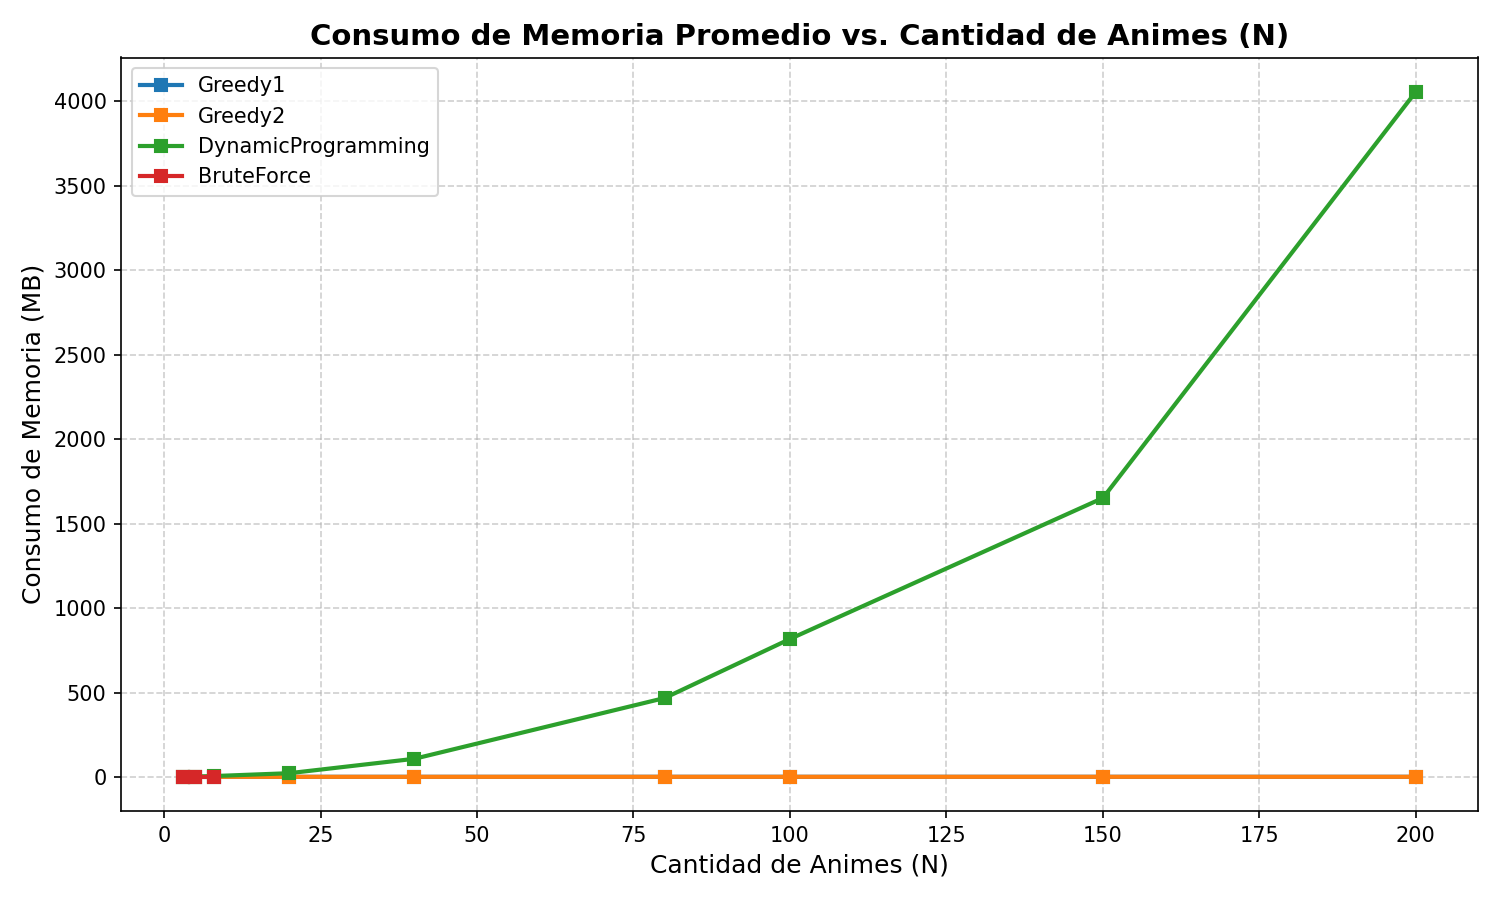
\includegraphics[width=0.70\textwidth]{../code/implementation/data/plots/memory_vs_n.png}
    \caption{Consumo de memoria promedio (MB) vs. Cantidad de animes ($N$).}
    \label{fig:memory}
\end{figure}

El uso de memoria de la Programación Dinámica experimenta un crecimiento cuadrático con respecto a los parámetros de entrada, llegando a requerir aproximadamente 3.94 GB de memoria RAM para $N=200$, debido a las dimensiones de la tabla DP de tamaño $(M+1) \times (E+1)$ donde $M=24244$ y $E=10641$. Por su parte, la Fuerza Bruta y los enfoques Greedy exhiben un uso plano y mínimo de memoria ($\approx 3.6$ MB), lo que ratifica la eficiencia espacial del análisis teórico.

\subsection{Análisis de Calidad de la Solución (Aproximación Heurística)}
La Figura~\ref{fig:quality} ilustra el ratio de calidad de las soluciones greedy respecto al óptimo teórico global obtenido por programación dinámica.

\begin{figure}[H]
    \centering
    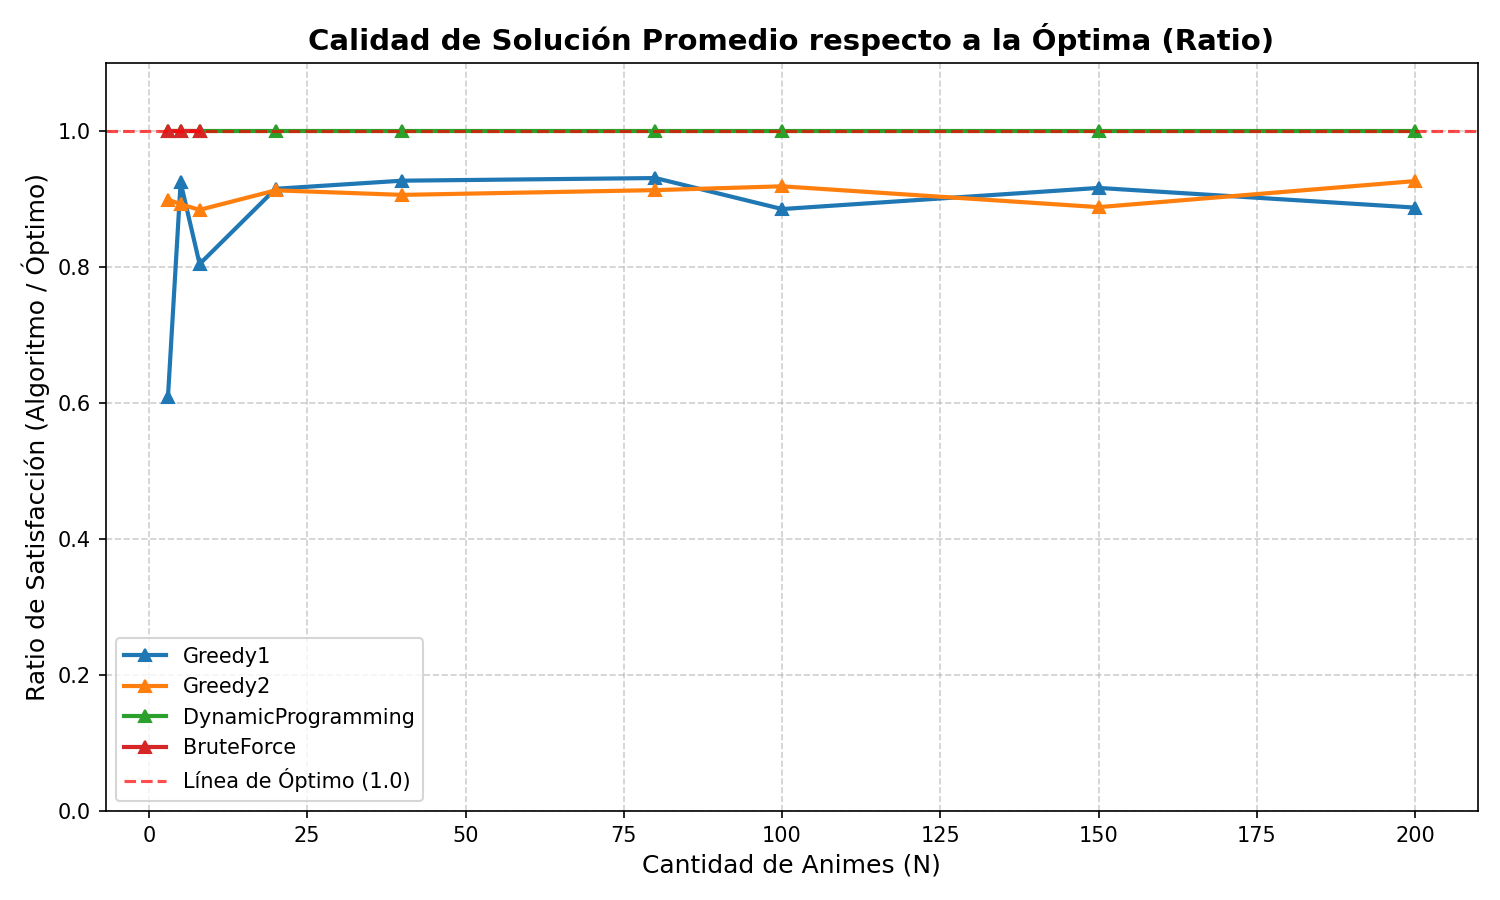
\includegraphics[width=0.70\textwidth]{../code/implementation/data/plots/quality_vs_n.png}
    \caption{Ratio de satisfacción promedio (Heurística / Óptimo) vs. Cantidad de animes ($N$).}
    \label{fig:quality}
\end{figure}

Se observa que la calidad promedio de Greedy 2 (Selección Marginal por Capítulo) se ubica consistentemente entre el 90\% y el 94\% del óptimo en las distintas escalas del experimento, superando a Greedy 1 (Densidad Global) en la mayoría de las instancias grandes. La flexibilidad de Greedy 2 para intercalar capítulos individuales permite una aproximación mucho más fina en los límites de la mochila bidimensional, mientras que Greedy 1 se ve penalizado al comprometer bloques rígidos completos, perdiendo oportunidades de rellenar la mochila en los bordes de las restricciones.

\section{Conclusiones}

Este estudio comprueba de forma experimental las fortalezas y compromisos teóricos de cada enfoque. La Programación Dinámica garantiza optimalidad absoluta al costo de un alto consumo de recursos, requiriendo 256.58 segundos y 3.94 GB de memoria en instancias con $N=200$. En escenarios de producción o sistemas embebidos donde la memoria y el tiempo de CPU son altamente restrictivos, la heurística Greedy 2 (Selección Marginal) constituye una excelente alternativa práctica, ofreciendo soluciones válidas con una calidad superior al 90\% del óptimo global con una latencia inferior a los 11 ms y un uso de memoria insignificante e independiente del tamaño de las restricciones.

\printbibliography

\end{document}
